\section{Pembahasan dan Tutorial Berbagai Macam Penanganan Error Proyek}

\subsection{Penanganan Error pada Python dan Flask}
\begin{enumerate}
  \item Contoh Kasus 1 : Penerapan fungsi sederhana yang dieksekusi dicommand prompt. Contoh pemanggilan fungsi apabila dieksekusi di CMD, seperti gambar \ref{fig:contohsederhana}

  \begin{figure}[!ht]
        \centerline{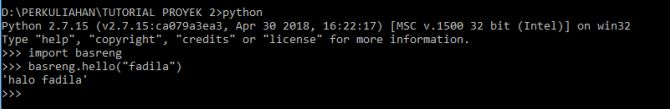
\includegraphics[width=0.70\textwidth]{figures/10/contohsederhana.jpg}}
	    \caption{Fungsi Sederhana}
	    \label{fig:contohsederhana}
  \end{figure}


ini adalah contoh untuk pengeksekusian file python yang berupa gunsi yang telah dibuat. Berikut langkah-langkahnya :
    \begin{itemize}
        \item Petama-tama masukkan kedalam directory tempat anda menyimpan file yang telah anda buat.
        \item kemudian pada directory tersebut ketik python
        \item Setelah masuk kedalam python silahkan masukkan file python basreng
    \end{itemize}

  \item Contoh kasus 2 : Kode pembawa sinyal gelombang otak (NeuroSky Mindwave EEG). Kodenya seperti contoh \ref{lst:coba}, silahkan tutorialnya diikuti terlebih dahulu.
\lstinputlisting[caption=Contoh kode untuk membaca sinyal gelombang otak,label={lst:coba}]{src/10/coba.py}
\end{enumerate}

